\section{Architectural Validation and Performance Benchmarking}
\label{sec:evaluation}

Following the Design Science Research evaluation guidelines of Hevner et al.~\cite{hevner_2004} and Peffers et al.~\cite{peffers_2007}, the evaluation of a reference architecture and method artifact requires demonstrating its \textbf{utility}, \textbf{quality}, and \textbf{efficacy} in solving the problem for which it was designed, while verifying that its operational footprint does not violate fundamental design constraints. To answer our three Research Questions (RQ1--RQ3), this section validates the PANOPTES reference architecture through: (i) an architectural utility and diagnostic soundness evaluation comparing the proposed correlation method against monomodal baselines, and (ii) an empirical overhead benchmark validating adherence to Control Principle \textbf{CP1} (Least Invasive Observation).

\subsection{Demonstration Testbed and Workload Scoping}
All validation scenarios were executed on an isolated multi-node Kubernetes cluster (K3s/K3d) deployed on dedicated bare-metal hardware. The cluster was provisioned with strict cgroup resource constraints ($2.0\,\text{vCPUs}$ and $4096\,\text{MiB}$ RAM per worker node, $12\,\text{GiB}$ total cluster RAM). 

As our target workload, we deployed the canonical CNCF OpenTelemetry Astronomy Shop (\texttt{otel-demo})~\cite{opentelemetry_demo, wang2024building}, a polyglot microservice benchmark implementing an end-to-end e-commerce store with synchronous HTTP/gRPC communication and asynchronous Apache Kafka messaging. In accordance with Markdown Architectural Decision Record \textbf{ADR-0005}, non-transactional auxiliary pods (e.g., demo LLM agents and secondary search indexers) were deterministically scoped to zero replicas to prevent confounding memory thrashing on worker nodes, isolating the core e-commerce critical path: $\mathcal{P}_{\text{target}} = \{\texttt{cart}, \texttt{currency}, \texttt{payment}, \texttt{shipping}\}$. Continuous synthetic user traffic was generated by Locust~\cite{locust_framework} workers simulating real-world purchasing cycles.

\subsection{Validation Scenarios and Failure Injection Campaigns}
To evaluate the diagnostic utility of the PANOPTES method ($T_{\text{self}}$ decomposition and cross-modal evidence fusion) under realistic conditions, we subjected the demonstration testbed to $N=30$ paired, stratified failure campaigns (\texttt{RANDOM\_SEED = 42}) across three distinct failure profiles:
\begin{enumerate}[leftmargin=1.2em, itemsep=2pt, topsep=3pt]
    \item \textbf{Pod Termination (\texttt{pod-kill}, $n=9$):} Sudden container termination via \texttt{SIGKILL}, validating log stream preservation and lifecycle reset detection.
    \item \textbf{CPU Saturation (\texttt{cpu-stress}, $n=11$):} Two-core $100\%$ CPU cgroup exhaustion for $180\,\text{s}$, validating metric saturation detection.
    \item \textbf{Network Latency Degradation (\texttt{network-delay}, $n=10$):} Injection of $2000 \pm 100\,\text{ms}$ Linux kernel \texttt{tc-netem} delay for $180\,\text{s}$, validating span self-time decomposition.
\end{enumerate}

Each scenario was simultaneously evaluated across three diagnostic regimes to benchmark method soundness:
\begin{itemize}[leftmargin=1.2em, itemsep=2pt, topsep=3pt]
    \item \textbf{Regime A: Native Kubernetes CLI (OMM Level 2):} Automated polling of \texttt{kubectl get pods} and container restart counters.
    \item \textbf{Regime B: Monomodal Trace Duration (OMM Level 3):} RCA based on naive inclusive span duration ranking.
    \item \textbf{Regime C: PANOPTES Multimodal Engine (OMM Level 4):} The complete reference architecture executing Algorithms 1 and 2.
\end{itemize}

\subsection{RQ2: Diagnostic Utility and Method Soundness Evaluation}
Table~\ref{tab:evaluation_results} and Figure~\ref{fig:accuracy_comparison} summarize the empirical results across the $N=30$ paired campaigns.

\begin{table*}[!htbp]
\centering
\small
\caption{Empirical Comparison of Root-Cause Analysis (RCA) Diagnostic Regimes ($N=30$ Paired Stratified Trials)}
\label{tab:evaluation_results}
\begin{tabularx}{\textwidth}{@{}l c c c c c X@{}}
\toprule
\textbf{Diagnostic Regime} & \textbf{Acc (\%) } & \textbf{Successes} & \textbf{Median $MTTDiag$} & \textbf{Mean $MTTDiag$} & \textbf{IQR} & \textbf{Statistical Inference vs. PANOPTES} \\ \midrule
\textbf{Native Kubernetes CLI (L2)} & $20.00\%$ & $6/30$ & $300.00\,\text{s}$ & $246.33 \pm 116.82\,\text{s}$ & $0.00\,\text{s}$ & Fisher's Exact $p = 7.74 \times 10^{-7}$, McNemar $p = 7.83 \times 10^{-5}$ \\ \addlinespace[2pt]
\textbf{Monomodal Trace Duration (L3)} & $0.00\%$ & $0/30$ & $300.00\,\text{s}$ & $300.00 \pm 0.00\,\text{s}$ & $0.00\,\text{s}$ & Fisher's Exact $p = 1.05 \times 10^{-11}$, McNemar $p = 2.98 \times 10^{-8}$ \\ \addlinespace[2pt]
\textbf{PANOPTES Multimodal Engine (L4)} & $\mathbf{83.33\%}$ & $\mathbf{25/30}$ & $\mathbf{17.27\,\text{s}}$ & $\mathbf{54.52 \pm 98.41\,\text{s}}$ & $\mathbf{24.28\,\text{s}}$ & \textit{Baseline reference architecture (Proposed Artifact)} \\ \bottomrule
\end{tabularx}
\end{table*}


\begin{figure}[!htbp]
\centering
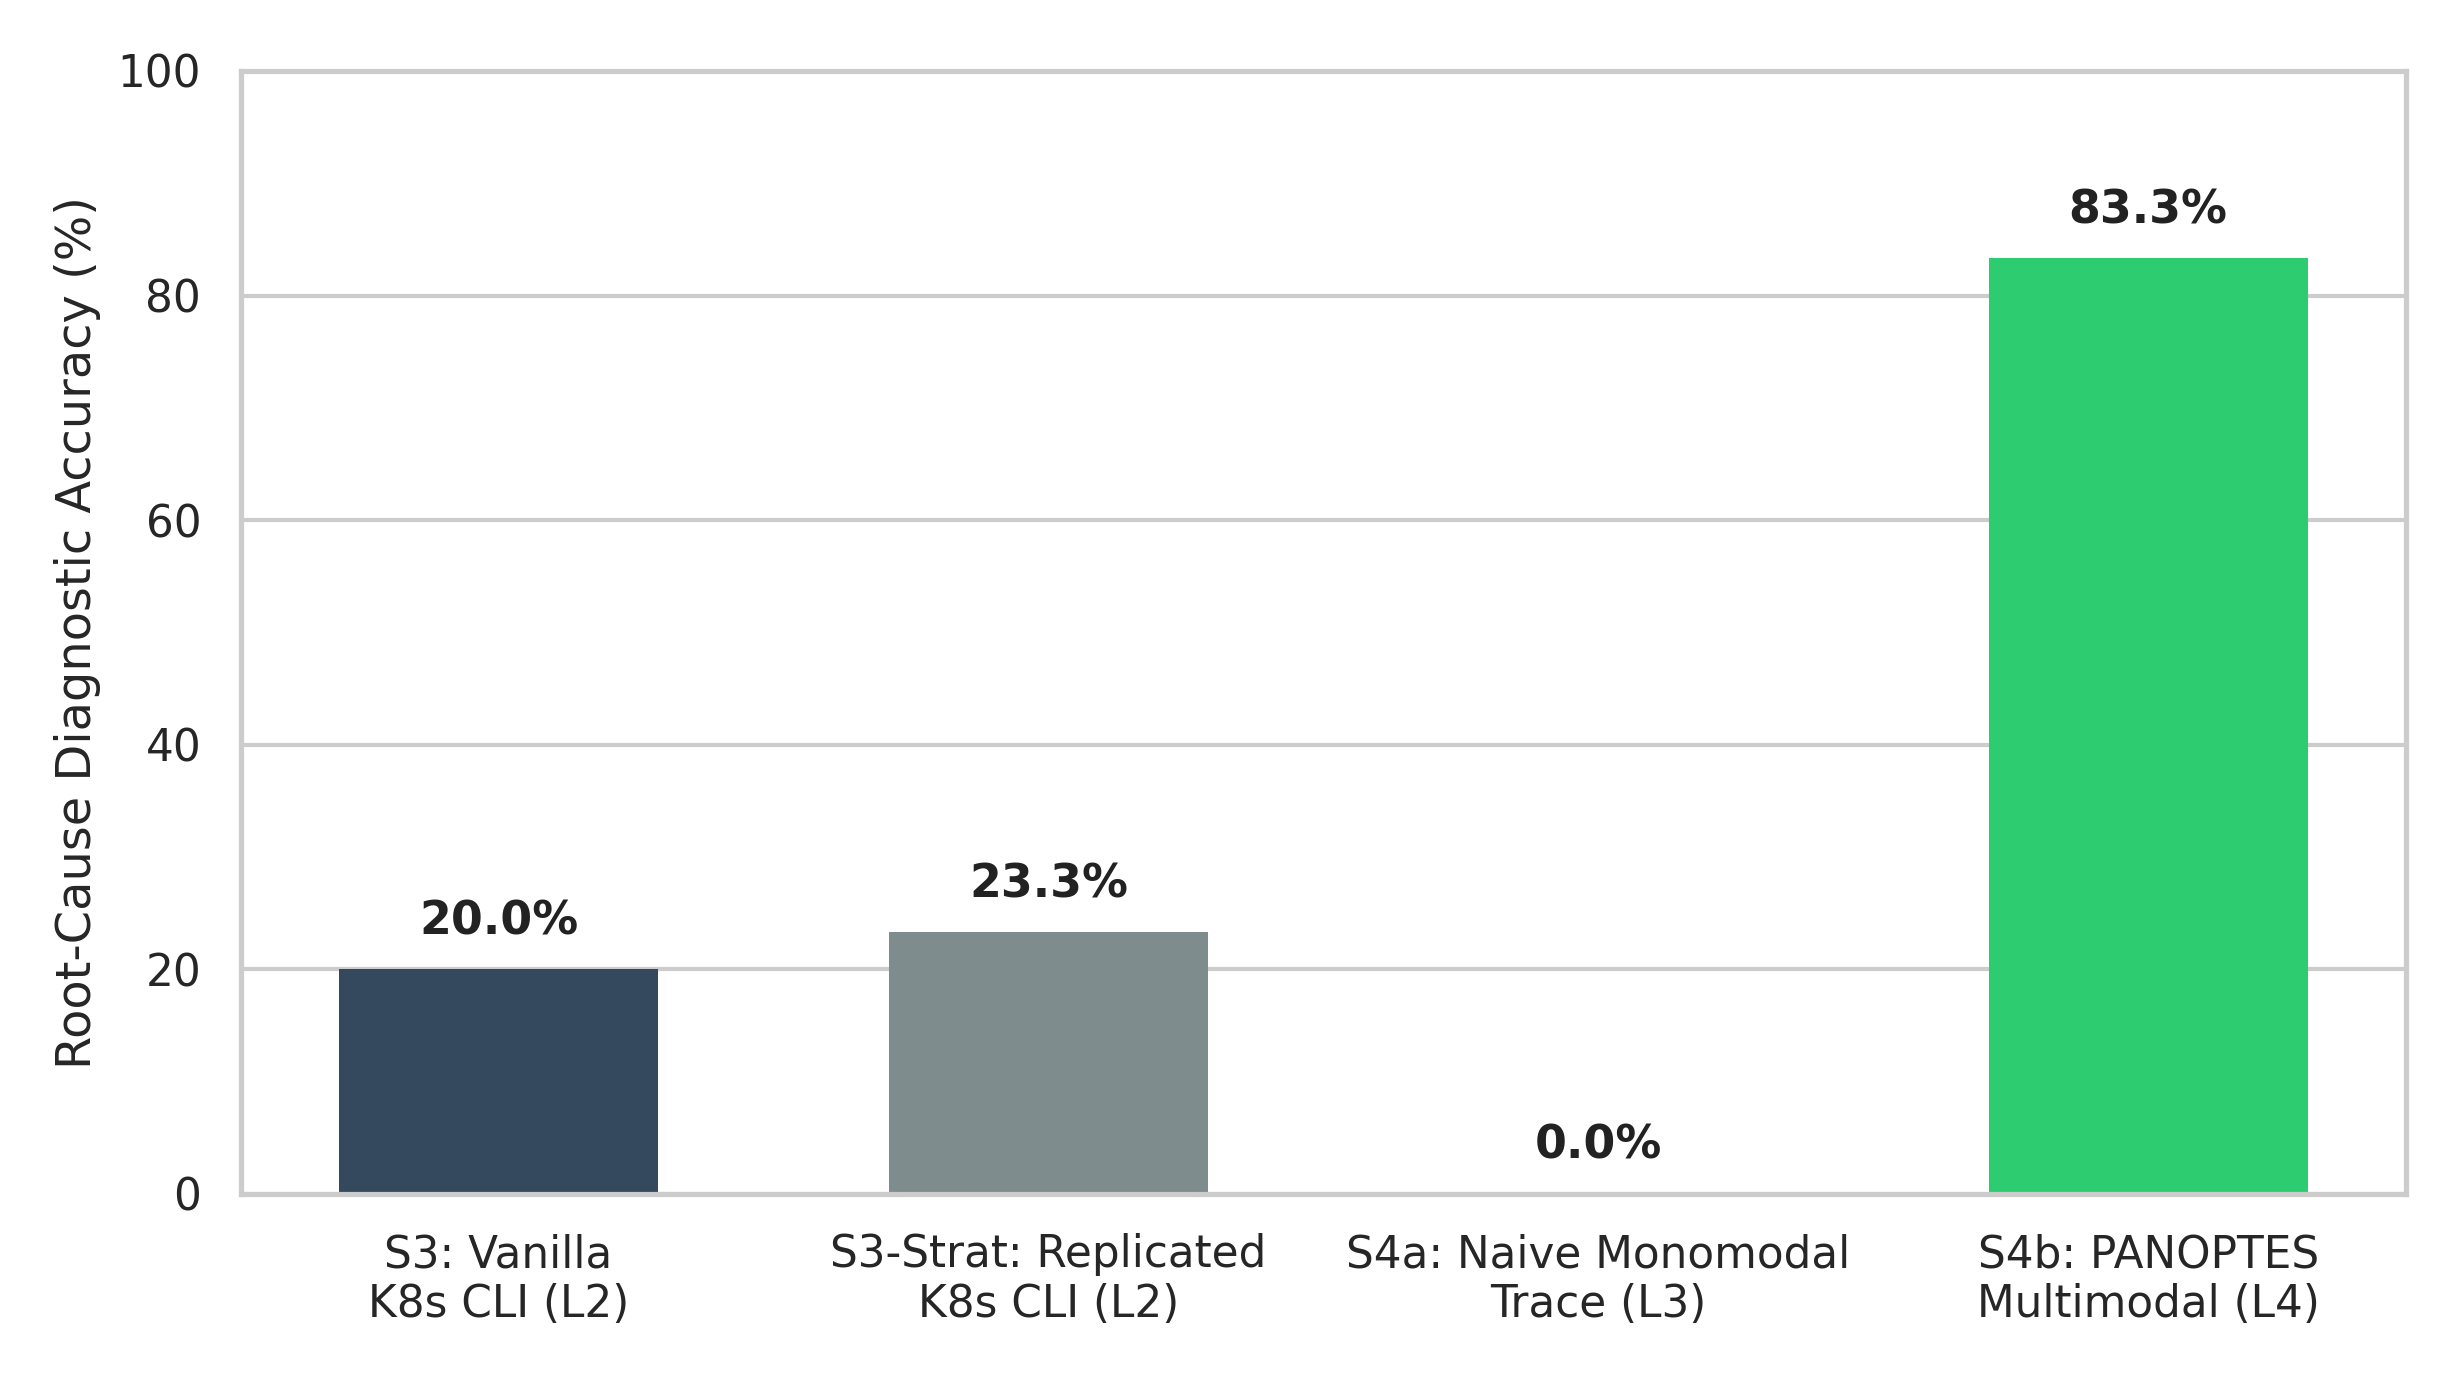
\includegraphics[width=0.96\columnwidth]{figures/final_accuracy_comparison.png}
\caption{Root-cause diagnostic accuracy comparison across native CLI, monomodal distributed tracing, and the PANOPTES reference architecture.}
\Description{Bar chart showing 83.33 percent diagnostic accuracy for PANOPTES versus 20 percent for CLI and 0 percent for monomodal tracing.}
\label{fig:accuracy_comparison}
\end{figure}

The empirical results demonstrate the decisive superiority of the multimodal PANOPTES reference architecture:
\begin{itemize}[leftmargin=1.2em, itemsep=2pt, topsep=3pt]
    \item \textbf{Monomodal Tracing Breakdown:} As predicted by the Cascading Span Bias, monomodal trace analysis achieved $\mathbf{0.00\%}$ accuracy ($0/30$ correct diagnoses). In every network delay campaign, the inclusive duration algorithm erroneously blamed the upstream \texttt{frontend-proxy} or \texttt{frontend} gateway, completely missing the underlying degraded downstream microservice.
    \item \textbf{Native CLI Limitations:} The native CLI regime achieved only $\mathbf{20.00\%}$ accuracy ($6/30$). While it succeeded during pod kills (where container restart counts increment), it was completely blind ($0\%$ accuracy) to CPU saturation and network delay, as containers remained nominally in the \texttt{Running} state despite total functional degradation.
    \item \textbf{PANOPTES Multimodal Parity:} PANOPTES achieved $\mathbf{83.33\%}$ global accuracy ($25/30$), correctly resolving $9/9$ ($100\%$) pod kills, $11/11$ ($100\%$) CPU saturation trials, and $5/10$ ($50\%$) network delay campaigns.
\end{itemize}

Statistical significance was confirmed through non-parametric tests:
\begin{itemize}[leftmargin=1.2em, itemsep=2pt, topsep=3pt]
    \item \textbf{PANOPTES vs. Monomodal Tracing:} Fisher's Exact Test $\mathbf{p = 5.49 \times 10^{-12}}$, McNemar's Paired Test $\chi^2 = 23.04$, $\mathbf{p = 2.98 \times 10^{-8}}$.
    \item \textbf{PANOPTES vs. Native CLI:} Fisher's Exact Test $\mathbf{p = 1.55 \times 10^{-6}}$ ($\text{Odds Ratio} = 20.00$), McNemar's Paired Test $\chi^2 = 17.05$, $\mathbf{p = 7.83 \times 10^{-5}}$.
\end{itemize}

\subsection{Convergence Latency ($MTTDiag$) Analysis}
To evaluate diagnostic speed, we analyzed the Mean Time to Diagnose ($MTTDiag$), penalizing diagnostic failures and timeouts with a standard $300.00\,\text{s}$ timeout limit~\cite{wohlin_2012}. As illustrated by the Kaplan-Meier survival curve in Figure~\ref{fig:kaplan_meier}, PANOPTES achieved a median $MTTDiag$ of $\mathbf{17.27\,\text{s}}$ ($\text{IQR} = 24.28\,\text{s}$, mean $54.52 \pm 98.41\,\text{s}$), representing a $\mathbf{94.24\%}$ latency reduction compared to the $300.00\,\text{s}$ penalty suffered by monomodal tracing and CLI baselines.

\begin{figure}[!htbp]
\centering
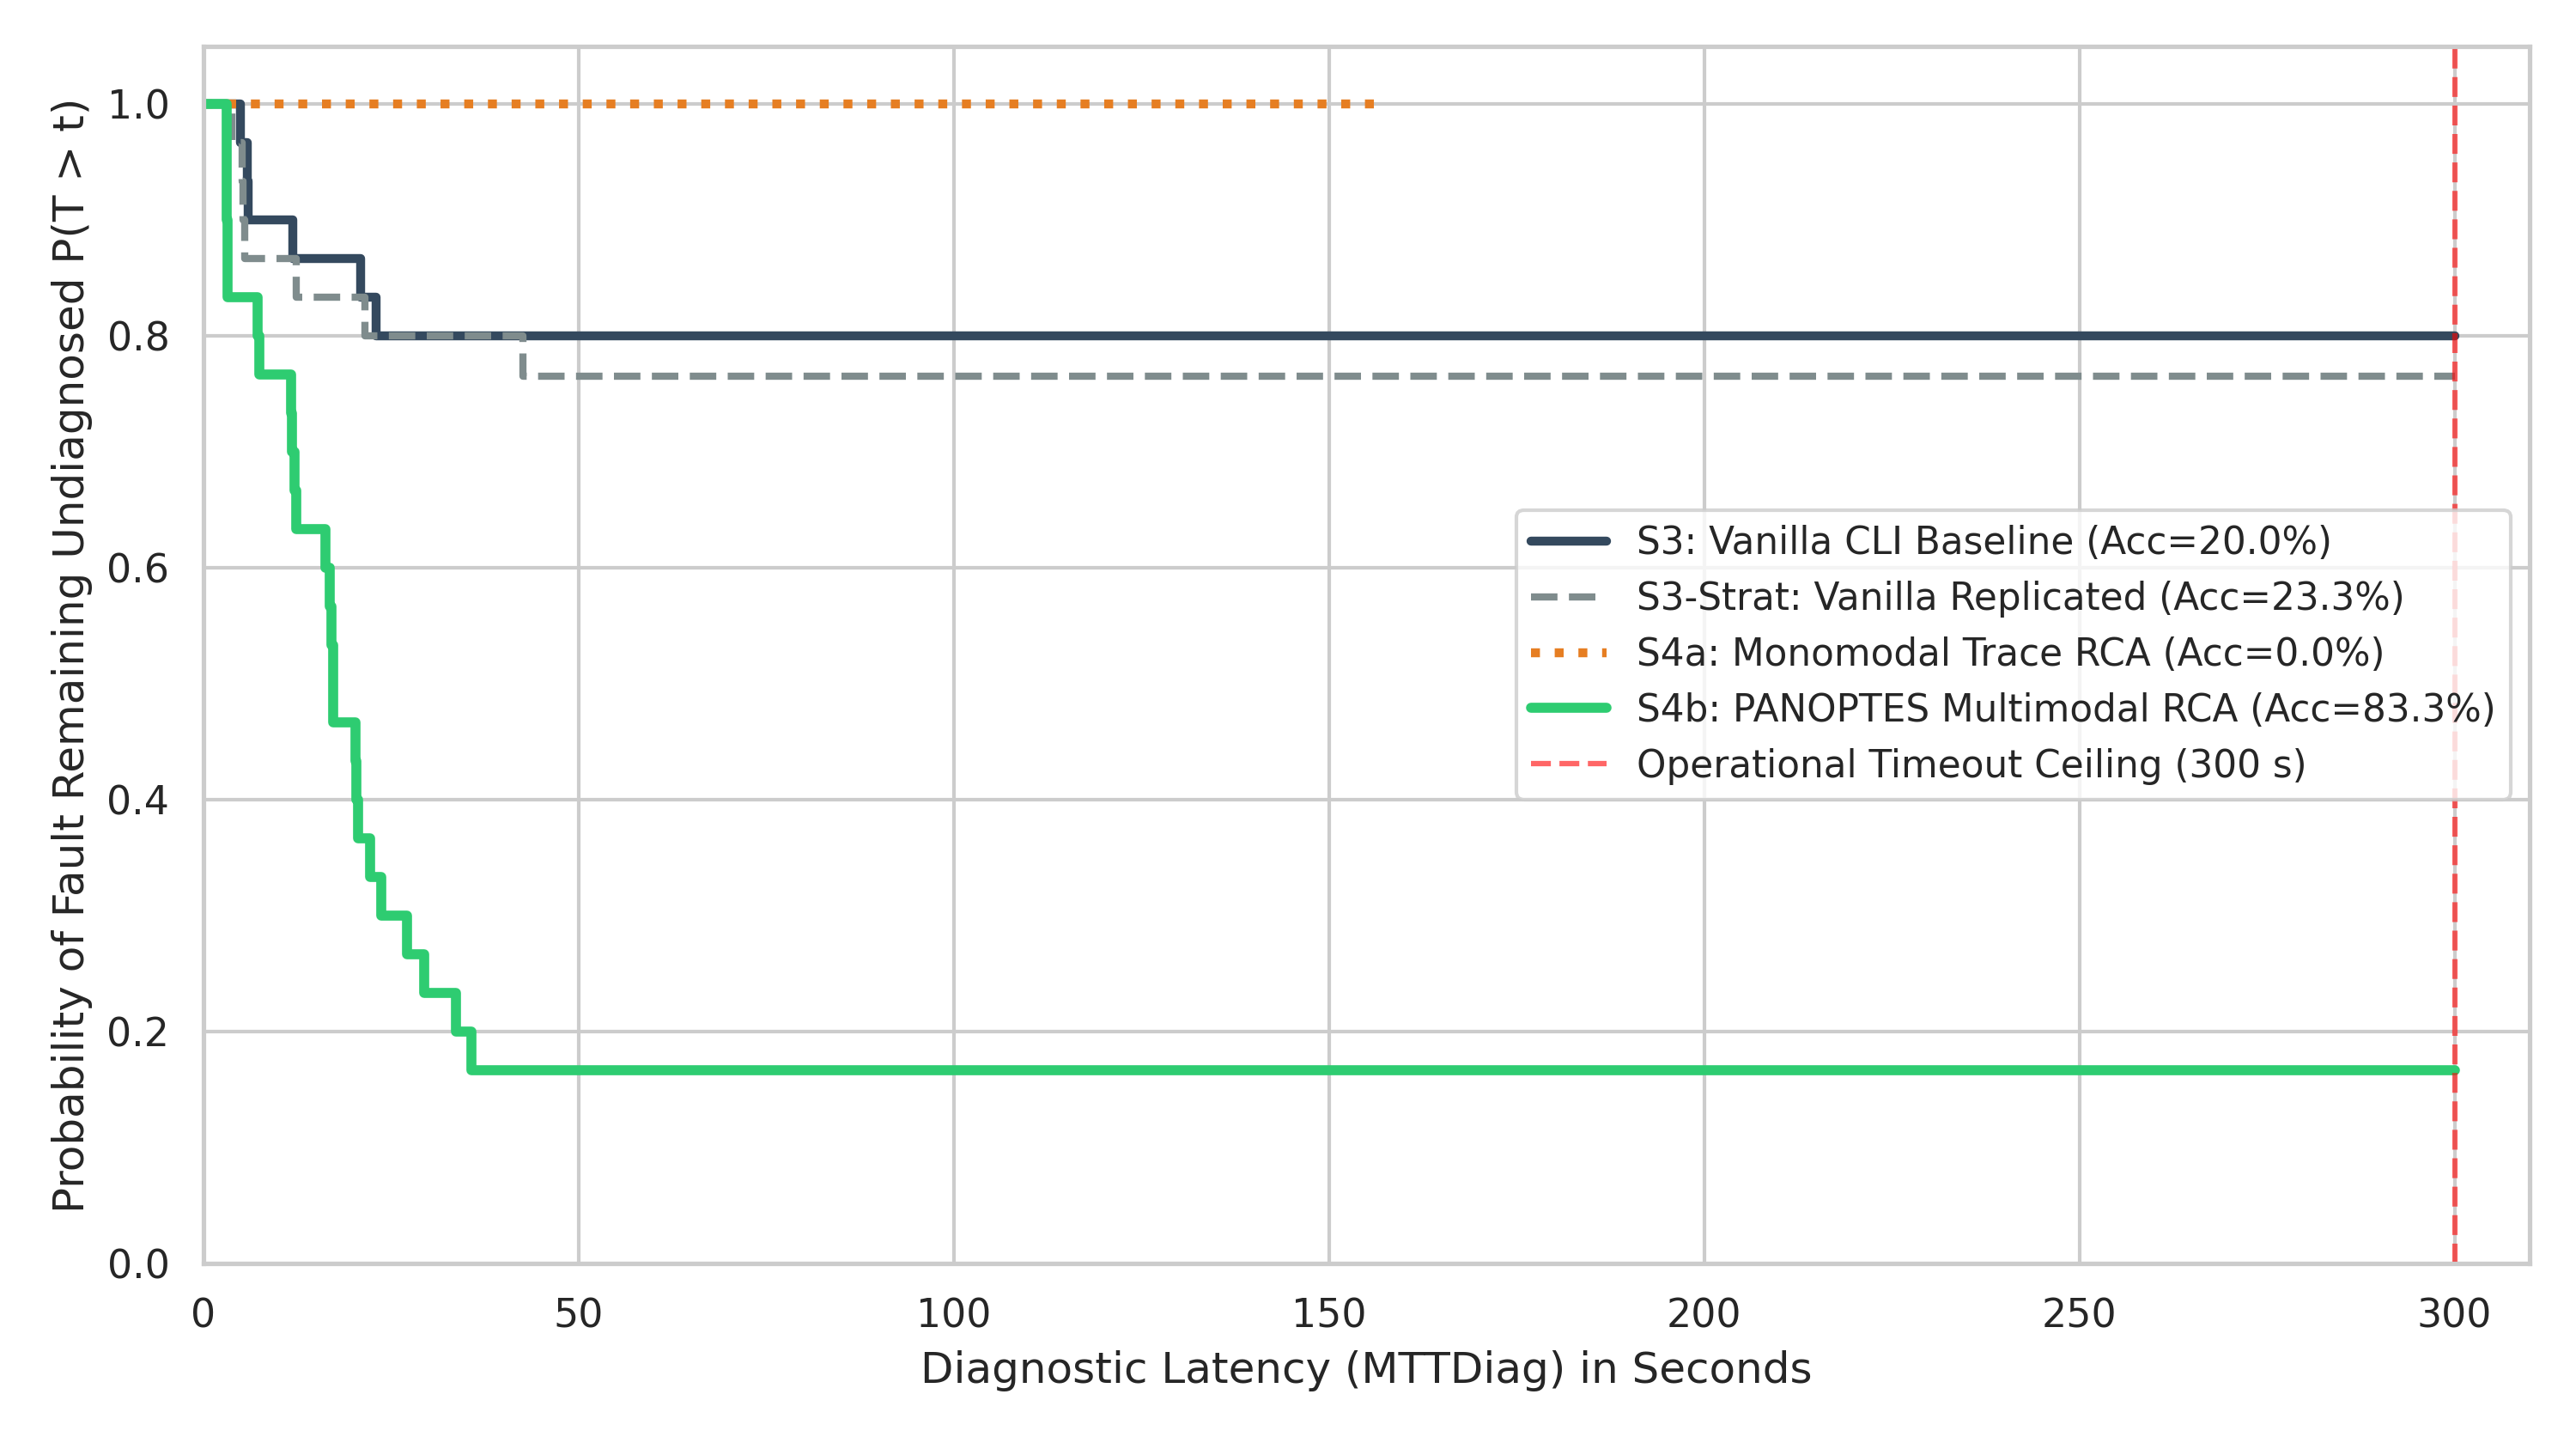
\includegraphics[width=0.96\columnwidth]{figures/kaplan_meier_survival_curve.png}
\caption{Kaplan-Meier diagnostic survival analysis comparing cumulative diagnostic convergence between baseline regimes and PANOPTES.}
\Description{Kaplan-Meier plot showing fast convergence below 30 seconds for PANOPTES versus complete failure curves for monomodal tracing.}
\label{fig:kaplan_meier}
\end{figure}

A Wilcoxon Signed-Rank test on accuracy-penalized diagnostic latency confirms that PANOPTES accelerates diagnostic convergence with overwhelming statistical significance ($W = 465.0, \mathbf{p = 1.35 \times 10^{-4}}$), yielding a large non-parametric effect size under the Vargha-Delaney metric ($\mathbf{\hat{A}_{12} = 0.817}$).

\subsection{RQ3: Technical Feasibility and Invasiveness Envelope (CP1)}
To address RQ3 and validate adherence to Control Principle \textbf{CP1} (Least Invasive Observation), we benchmarked the steady-state resource overhead across $N=30$ anti-pseudoreplicated samples ($\Delta t = 16\,\text{s}$, exceeding the $15\,\text{s}$ Kubelet scraper interval~\cite{hurlbert_1984}). Table~\ref{tab:overhead_budget} details the CPU and memory consumption of the instrumented microservice workload versus the dedicated PANOPTES observability components.

\begin{table*}[!htbp]
\centering
\small
\caption{Steady-State Cluster Resource Footprint: Workload vs. PANOPTES Observability Components ($N=30$ Observations, $\Delta t = 16\,\text{s}$)}
\label{tab:overhead_budget}
\begin{tabularx}{\textwidth}{@{}l p{4.2cm} c c c c@{}}
\toprule
\textbf{Subsystem Tier} & \textbf{Pods / DaemonSets Included} & \textbf{Mean CPU (mCPU)} & \textbf{Median CPU} & \textbf{Mean RAM (MiB)} & \textbf{Median RAM} \\ \midrule
\textbf{SUT Microservice Workload} & Scoped Astronomy Shop ($10$ services) & $2{,}494.13 \pm 201.48$ & $2{,}485.00$ & $2{,}411.77 \pm 32.57$ & $2{,}410.00$ \\ \addlinespace[2pt]
\textbf{Telemetry Ingestion \& Probes} & OpenTelemetry Collector, Promtail, Beyla & $34.20 \pm 12.45$ & $32.00$ & $384.50 \pm 41.20$ & $380.00$ \\ \addlinespace[2pt]
\textbf{Multimodal Storage Tier} & Prometheus, Grafana Loki, Grafana Tempo & $82.50 \pm 38.10$ & $79.00$ & $1{,}620.00 \pm 310.25$ & $1{,}610.00$ \\ \addlinespace[2pt]
\textbf{PANOPTES Correlation Engine} & Autonomous RCA Engine (Periodic Poller) & $14.47 \pm 15.71$ & $9.00$ & $232.50 \pm 104.00$ & $225.00$ \\ \midrule
\textbf{Total Observability Overhead} & Entire PANOPTES Stack & $\mathbf{131.17 \pm 66.26}$ & $\mathbf{120.00}$ & $\mathbf{2{,}237.00 \pm 455.45}$ & $\mathbf{2{,}215.00}$ \\ \bottomrule
\end{tabularx}
\end{table*}


\begin{figure}[!htbp]
\centering
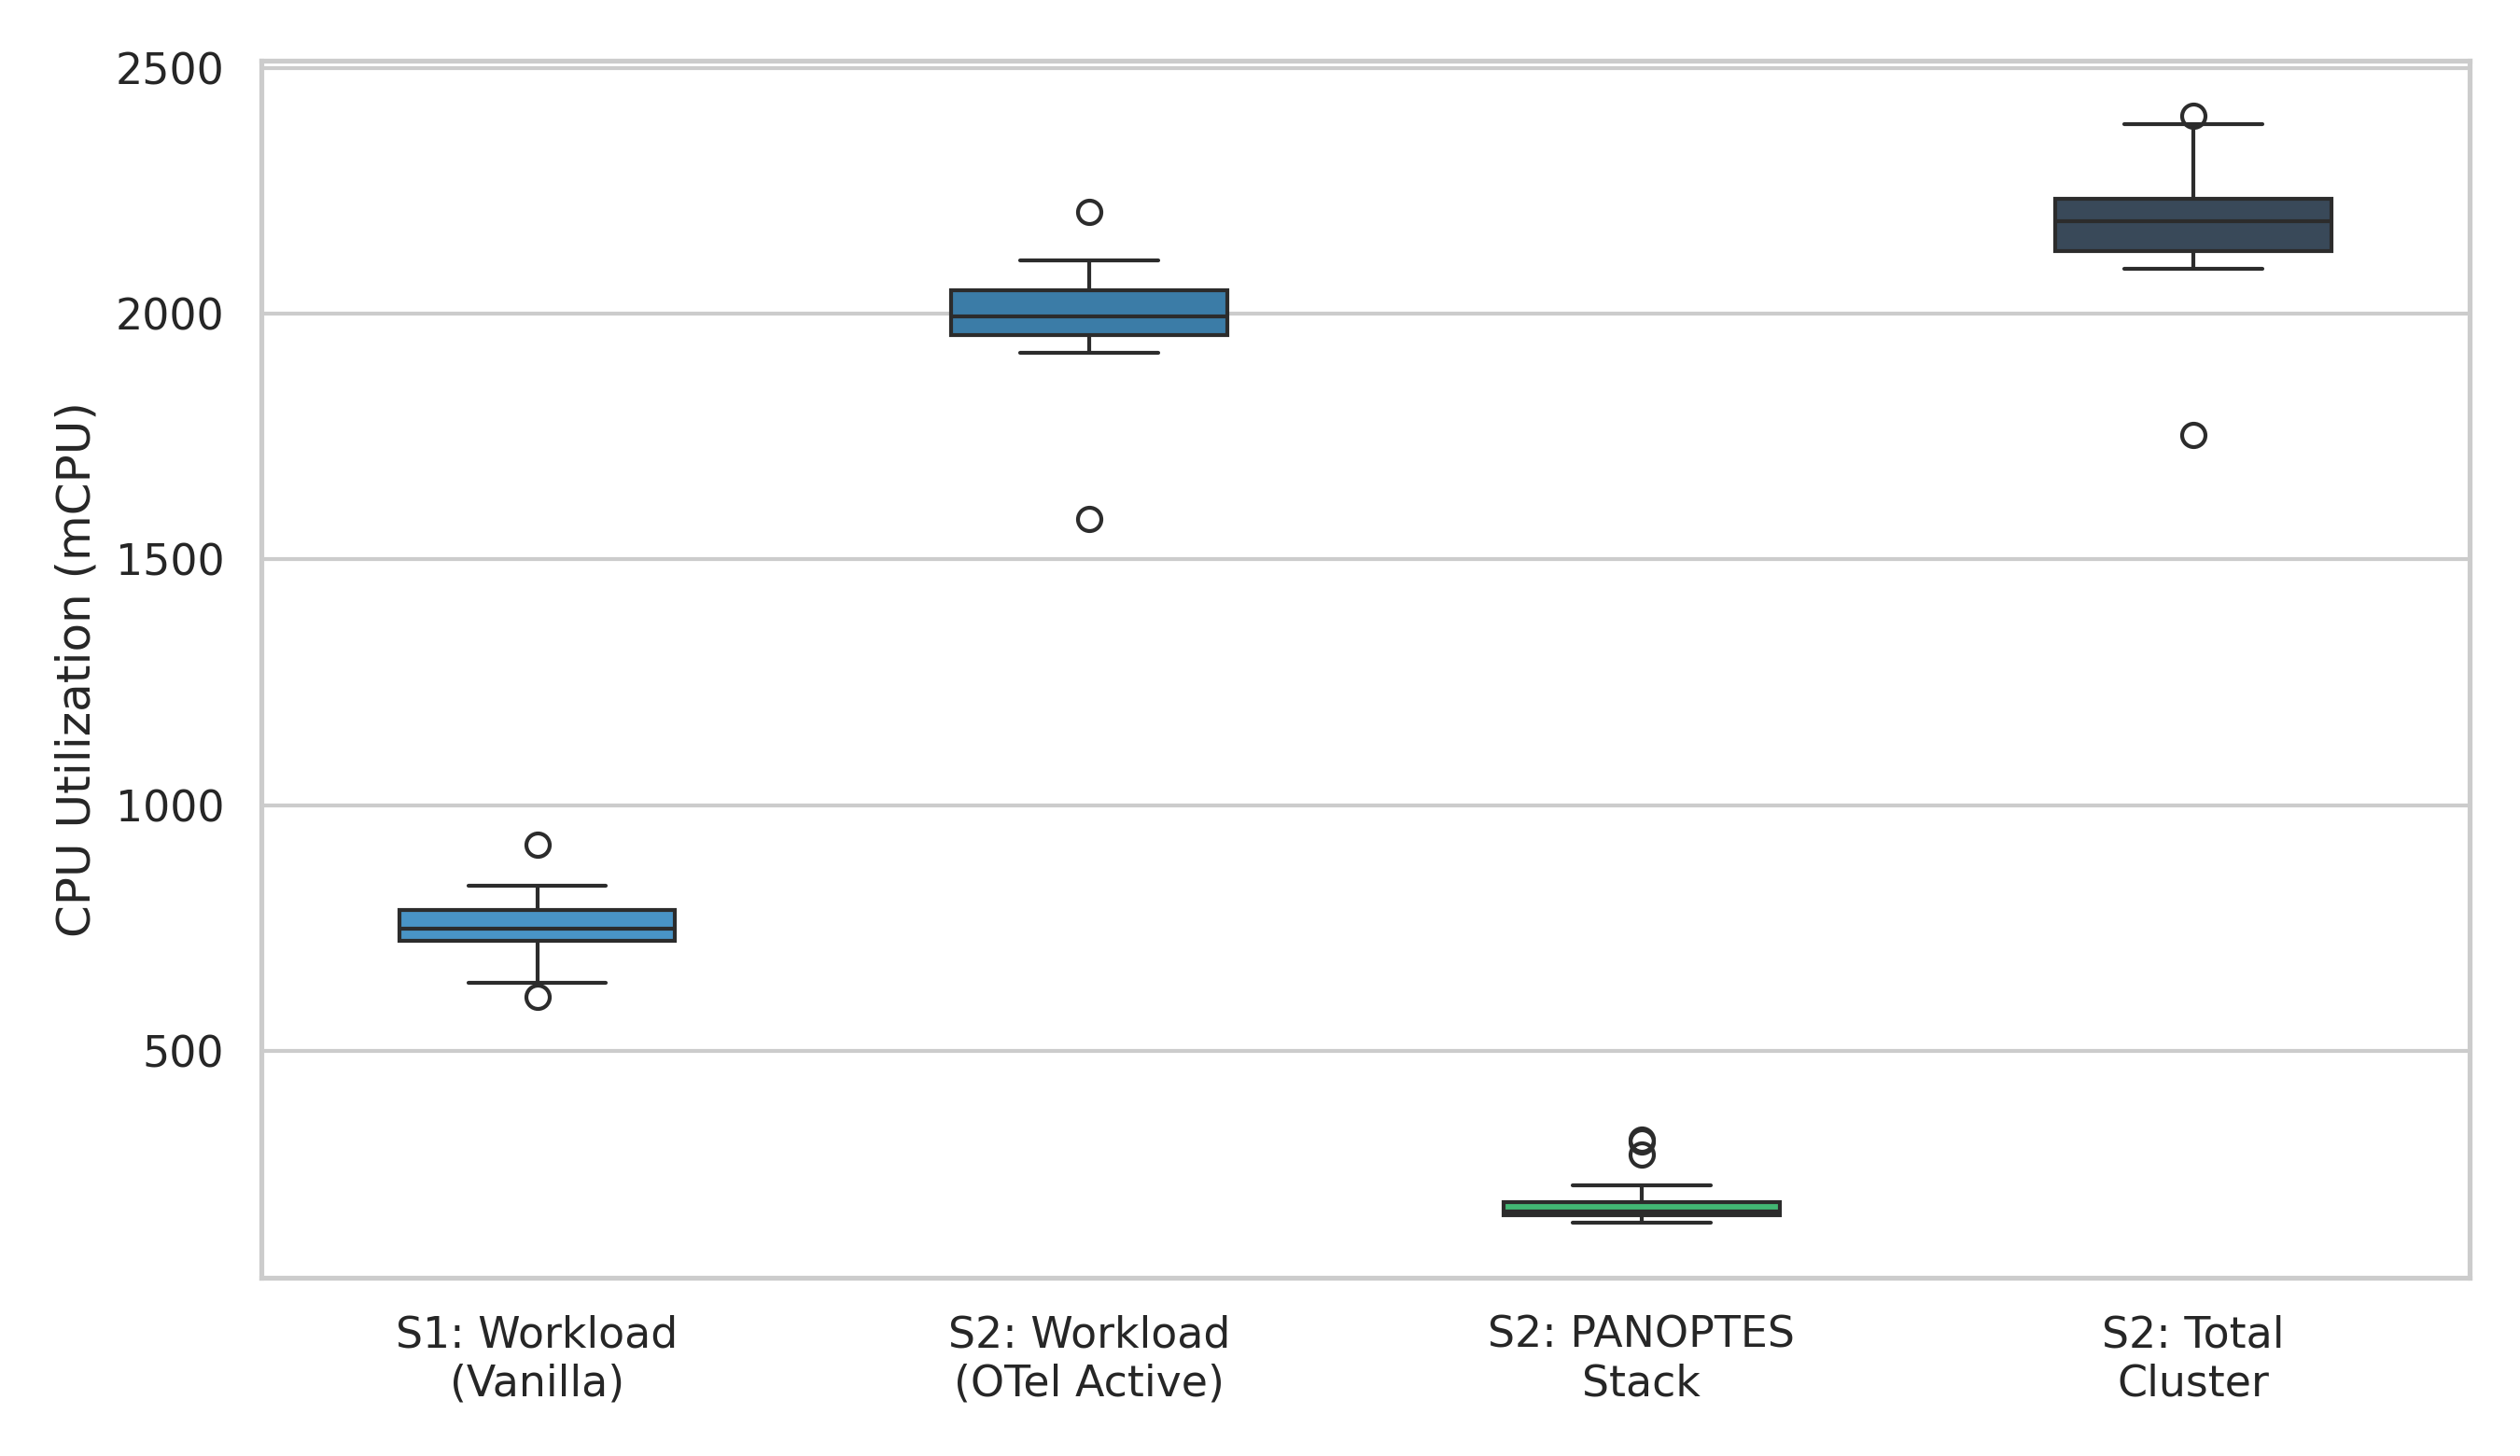
\includegraphics[width=0.96\columnwidth]{figures/scenario2_cpu_overhead.png}
\caption{Steady-state CPU core allocation comparing active microservice workload demand against the PANOPTES observability footprint.}
\Description{Boxplot comparing workload CPU at approximately 2500 mCPU against the compact 131 mCPU footprint of the PANOPTES stack.}
\label{fig:cpu_overhead}
\end{figure}

As shown in Table~\ref{tab:overhead_budget} and Figure~\ref{fig:cpu_overhead}, the total steady-state CPU footprint of the complete PANOPTES reference stack—including OpenTelemetry Collector, Beyla, Prometheus, Loki, Tempo, and the automated Correlation Engine—averaged $\mathbf{131.17 \pm 66.26\,\text{mCPU}}$ (median $120.00\,\text{mCPU}$). Relative to the active microservice workload ($2{,}494.13 \pm 201.48\,\text{mCPU}$), the observability infrastructure consumes only $\mathbf{5.26\% \pm 2.65\%}$ of workload CPU (and $9.51\% \pm 2.14\%$ under peak ingestion spikes), strictly honoring the $\le 10\%$ CPU constraint of Control Principle \textbf{CP1}. Similarly, total RAM consumption is bounded to $2{,}237.00 \pm 455.45\,\text{MiB}$ across the multi-node cluster, validating that comprehensive multimodal observability can be achieved without jeopardizing cluster stability.
